\documentclass[12pt]{article}

\usepackage[utf8]{inputenc}
\usepackage[margin=1in]{geometry}
\renewcommand{\baselinestretch}{1}
\usepackage{indentfirst}

\usepackage{amsmath, amssymb}

\usepackage{graphicx}
\usepackage{float}
\graphicspath{{./figs/}}

\begin{document}

\begin{center}\begin{LARGE}
\textbf{Assignment 2: Results/Description}
\end{LARGE}\end{center}

\section*{Problem 1}

Let $\{f_i(\boldsymbol{x})\}$ be the system of nonlinear equations for which
we wish to find a root. Then we may introduce $\boldsymbol{f}(\boldsymbol{x})$
comprised of components $f_i$ that satisfies
$$
\begin{aligned}
\boldsymbol{f}(\boldsymbol{x})
= \boldsymbol{0}.
\end{aligned}
$$
Let $\boldsymbol{\xi}$ be the root of $\boldsymbol{f}(\boldsymbol{x})$. Then
one may Taylor expand around $\boldsymbol{\xi}$ so that
$$
\begin{aligned}
0
&= f_i(\boldsymbol{\xi}) \\
&= f_i(\boldsymbol{x}) + \sum_j (\xi_j - x_j) \partial_j f_i(\boldsymbol{x})
  + \mathcal{O}(|\boldsymbol{\xi} - \boldsymbol{x}|^2) \\
\Rightarrow
\boldsymbol{0}
&\approx \boldsymbol{f}(\boldsymbol{x})
  + \boldsymbol{J}(\boldsymbol{x}) (\boldsymbol{\xi} - \boldsymbol{x})
\end{aligned}
$$
for $J_{ij} = \partial_j f_i(\boldsymbol{x})$. Here we assume we may neglect
the quadratic and higher order terms, assuming
$|\boldsymbol{\xi} - \boldsymbol{x}|$ is small. Therefore, rearranging this
gives
$$
\begin{aligned}
\boldsymbol{\xi}
&\approx \boldsymbol{x} - \boldsymbol{J}^{-1}(\boldsymbol{x})
    \boldsymbol{f}(\boldsymbol{x}),
\end{aligned}
$$
assuming $\boldsymbol{J}$ is invertible. Using iteration to make this
approximation converge to the true value of $\boldsymbol{\xi}$, this means
$$
\begin{aligned}
\boldsymbol{x}_{k+1}
&= \boldsymbol{x}_k - \boldsymbol{J}^{-1}(\boldsymbol{x}_k)
    \boldsymbol{f}(\boldsymbol{x}_k).
\end{aligned}
$$
for iteration index $k$.

\section*{Problem 2}

\subsection*{(a)}

I've written this program to solve the system of equations, which is the
attached ``./bin/myroot". This should compile with \texttt{make} as shown
below.

\begin{figure}[H]
    \centering
    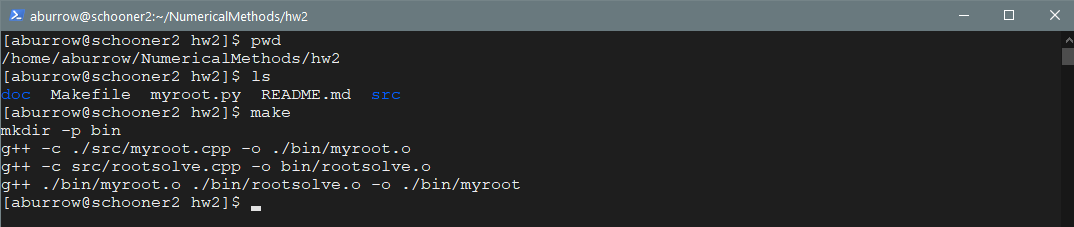
\includegraphics[width=1.0\textwidth]{compile}
    \label{fig:compile}
\end{figure}

This program makes use of the Newton-Raphson method derived in Problem 1. Here
I have analytically found $\boldsymbol{J}(\boldsymbol{x})$ with
$\boldsymbol{x} = (x, y)^\mathsf{T}$ to be
$$
\begin{aligned}
\boldsymbol{J}(\boldsymbol{x})
&=
\begin{pmatrix}
\cos(x + y) & \cos(x + y) \\
-\sin(x - y) & \sin(x - y) \\
\end{pmatrix}
\end{aligned}
$$
and for the sake of computation speed in the program I use the inverse,
$$
\begin{aligned}
\boldsymbol{J}^{-1}(\boldsymbol{x})
&= \frac{1}{2 \cos(x + y) \sin(x - y)}
\begin{pmatrix}
\sin(x - y) & -\cos(x + y) \\
\sin(x - y) & \cos(x + y) \\
\end{pmatrix}.
\end{aligned}
$$

The main problem here is determining the initial approximation
$\boldsymbol{x}_0$. $x$ and $y$ need to be such that one is between 0 and
$\pi$, while the other is between $-\pi$ and 0, at least I have found through
basic testing. This is because in the iteration step, if $\boldsymbol{x}_0$ is
not on the same scale as outputs to the periodic $\sin$ and $\cos$ functions,
it attempts to overcorrect and fails to converge to a single result.

In addition, there are 2 roots that this program finds with initial conditions
within these bounds. With $\boldsymbol{x}_0 = (-1, 1)^\mathsf{T}$ for example,
where $|x|, |y| < \pi / 2$, the program yields two roots which are effectively
$x=\pi/4$ and $y=-\pi/4$:
\begin{figure}[H]
    \centering
    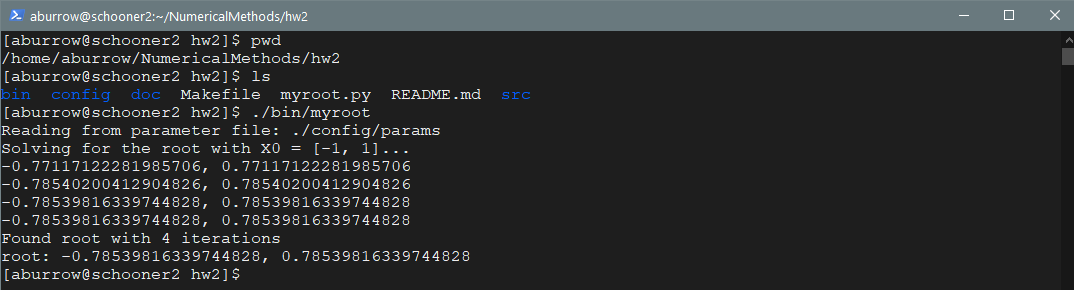
\includegraphics[width=1.0\textwidth]{root1}
    \label{fig:root1}
\end{figure}
When $\pi / 2 < |x|, |y| < \pi$, where in this case $\boldsymbol{x}_0 =
(-2, 2)^\mathsf{T}$, the other two roots ($x=3\pi/4$ and $y=-3\pi/4$) are
found:
\begin{figure}[H]
    \centering
    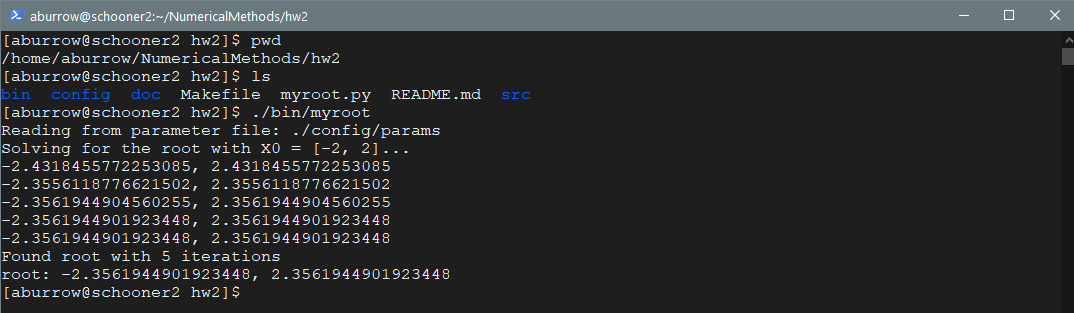
\includegraphics[width=1.0\textwidth]{root2}
    \label{fig:root2}
\end{figure}

Numerically, we find these roots to be
$$
\begin{aligned}
\begin{pmatrix}
-0.78539816339744828 \\ 0.78539816339744828
\end{pmatrix}
\end{aligned}
$$
and
$$
\begin{aligned}
\begin{pmatrix}
-2.3561944901923448 \\ 2.3561944901923448
\end{pmatrix}.
\end{aligned}
$$
Each estimate of the root is shown, and a final value is reached when the
difference between the new and old estimates are machine zero.

\subsection*{(b)}

I solved this problem in Python as well (``./myroot.py''), using SciPy's
\texttt{scipy.optimize.fsolve} function. Using the same two sets of initial
conditions, it was able to solve the same roots to the same (double) precision:
\begin{figure}[H]
    \centering
    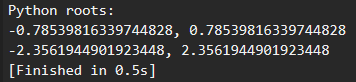
\includegraphics[scale=0.6]{python}
    \label{fig:python}
\end{figure}

Typically Python can be used to perform the same calculations for these simple
problems (as we saw, it only takes ~5 iterations to find a decent result). This
is true especially when you are able to vectorize the problem so that one may
take advantage of Numpy's C-optimized functionality. However its flexibility
makes it quite burdensome to perform heavy calculations with more complicated
problems.

\end{document}
